
%(BEGIN_QUESTION)
% Copyright 2005, Tony R. Kuphaldt, released under the Creative Commons Attribution License (v 1.0)
% This means you may do almost anything with this work of mine, so long as you give me proper credit

We know that the output rate-of-change of an integrator circuit is proportional to the input voltage:

$$\includegraphics[width=15.5cm]{i01567x01.eps}$$

$$V_{in} \propto {dV_{out} \over dt}$$

But how do we turn this proportionality into an exact equality, so that it accounts for the values of $R$ and $C$?  Although the answer to this question is easy enough to simply look up in an electronics reference book, it would be great to actually derive the exact equation from your knowledge of electronic component behaviors!  Here are a couple of hints:

$$I = {V \over R} \hbox{\hskip 50pt} i = C {dv \over dt}$$

\underbar{file i01567}
%(END_QUESTION)





%(BEGIN_ANSWER)

$${dV_{out} \over dt} = - {V_{in} \over RC}$$

$$\hbox{. . . or . . .}$$

$$V_{out} = - {1 \over RC} \int V_{in} \> dt$$

\vskip 10pt

Follow-up question: why is there a negative sign in the equation?

%(END_ANSWER)





%(BEGIN_NOTES)

The two ``hint'' equations given at the end of the question beg for algebraic substitution, but students must be careful which variable(s) to substitute!  Both equations contain an $I$, and both equations also contain a $V$.  The answer to that question can only be found by looking at the schematic diagram: do the resistor and capacitor share the same current, the same voltage, or both?

%INDEX% Electronics review: integrator circuit

%(END_NOTES)


